\documentclass[12pt, a4paper]{article}

\usepackage{blindtext}
\usepackage{titlesec}
\usepackage[czech]{babel}
\usepackage{biblatex}
\usepackage{csquotes}
\usepackage{amsmath}
\addbibresource{zdroje.bib}

\usepackage{graphicx}

\graphicspath{files/}

\usepackage{tocloft}
\usepackage{caption}
\renewcommand{\cftsecleader}{\cftdotfill{\cftdotsep}}

\begin{document}

\nocite{csob-podnikatelsky-plan}
\author{Jan Prokůpek, Miroslav Sklenář}
\title{\textbf{Podnikatelské záměry}}
\date{}

\maketitle

\pagebreak

\tableofcontents

\pagebreak

\section{Shrnutí}

\subsection{Jméno a místo podnikání}
Jedná se o fiktivní firmu \textbf{Hats for Cats s.r.o.} se sídlem v Brně.

\subsection{Obchodní koncept}
Hats for Cats je originální značka specializující se na výrobu a prodej stylových, pohodlných a funkčních čepic pro kočky. 
Naším cílem je přinést do světa mazlíčků špetku originality a elegance, která potěší jak majitele, tak jejich kočičí společníky.

\subsection{Prodávaný produkt/služba}
Nabízíme ručně vyráběné čepice pro kočky v různých stylech a velikostech, 
které jsou přizpůsobeny pohodlí a bezpečnosti zvířete. 
Produkty zahrnují sezónní kolekce (zimní čepice, letní kloboučky) i tematické modely (vánoční, narozeninové, apod.),
či čepice kompletně na míru.

\subsection{Plněná potřeba na trhu}
V současnosti chybí na trhu esteticky atraktivní a funkční doplňky pro kočky, které by splňovaly požadavky majitelů na kvalitu a design. Hats for Cats vyplňuje tuto mezeru a oslovuje rostoucí komunitu milovníků koček, kteří hledají jedinečné produkty pro své mazlíčky.

\subsection{Konkurenční výhoda}
Naše konkurenční výhody spočívají v unikátním designu, použití kvalitních a hypoalergenních materiálů a důrazu na ruční výrobu. Dále se zaměřujeme na silný marketing na sociálních sítích, který osloví cílovou skupinu mladých a kreativních zákazníků.
Mezi existující alternativy patří levné a nekvalitní produkty z Číny, které nejsou přizpůsobeny potřebám zvířat a často mohou
způsobit zdravotní problémy kočkám, nebo tržiště jako Etsy.

\subsection{Ziskovost}
Očekáváme, že během prvního roku dosáhneme návratnosti investic díky 
nízkým provozním nákladům 
a atraktivní marži na našich produktech.

\subsection{Momentální situace}
Projekt je ve fázi příprav, zahrnující tvorbu prvních prototypů, 
testování na trhu a sestavování marketingové kampaně.

\subsection{Účel podnikatelského plánu}
Podnikatelský plán slouží k získání investice na zahájení výroby, 
marketingovou propagaci a rozšíření distribuční sítě.

\subsection{Potřeba investice}
Základní vklad na zahájení výroby, marketing, tvorbu webové stránky, materály,
pronájem prostor a další, bude činit cca 3 000 000 Kč.

\section{Představení společnosti}
Společnost \textbf{Hats for Cats s.r.o.} byla založena 2 fyzickými osobami,
které podnikají dle živnostenského oprávnění. Dle společenské smlouvy
každý z majitelů vlastní 50\% podíl na společnosti a má rovnocenný podíl v zisku.
Jednatelem společnosti je Jan Prokůpek.

\vspace{10pt}

\noindent Hats for Cats s.r.o. je společnost zaměřená na výrobu a prodej různých typů čepic pro kočky.
Nabízí ručně vyráběné produkty, které jsou uzpůsobeny několika velikostem, tak aby seděly na většinu koček.
Lze si také nechat vyrobit čepici na míru.

\pagebreak

\section{Podnikatelský projekt}

Hats for Cats se zaměřuje na výrobu, prodej a distribuci módních doplňků pro domácí mazlíčky, konkrétně kočky. 
Hlavní obory podnikání zahrnují:

\begin{enumerate}
  \item Výroba textilních doplňků. Jedná se o ekonomickou činost s kódem CZ-NACE 14.19.
  \item Maloobchod a e-commerce - kód CZ-NACE 47.91.
\end{enumerate}

\subsection{Vstupní předpoklady}

\subsubsection{Oprávnění k provozování podniku}
\begin{itemize}
  \item Získání potřebného kapitálu.
  \item Založení společnosti s ručením omezeným (s.r.o.):
  \begin{itemize}
    \item Zápis do obchodního rejstříku.
    \item Zaplacení správního poplatku.
    \item Získání IČO.
    \item Notářsky ověřený zápis společenské smlouvy mezi společníky.
  \end{itemize}
  \item{Registrace k daním} - pokud bude obrat vyšší než 2 mio. Kč, bude nutné se registrovat k dani z přidané hodnoty.
\end{itemize}

\subsubsection{Požadavky na zaměstnance}
Zaměstnanci by měli být schopni ručně šít a zpracovávat textilní materiály.

\subsubsection{Materiální a technické vybavení}
\begin{itemize}
  \item Prostory pro výrobu, skladování a administrativu.
  \item Šicí stroje, nůžky, střihové šablony, materiály a ostatní vybavení pro výrobu.
  \item Zázemí pro administrativu a marketing(počítač, tiskárna atd.).
\end{itemize}

\subsection{Organizačně-právní forma podnikání}
Podnik bude již od počátku fungovat jako společnost s ručením omezeným (s.r.o.).
Tato forma podnikání byla zvolena pro možnost oddělení osobního majetku majitelů od majetku společnosti.
Zároveň umožňuje získání investic od externích investorů.

\subsection{Stadium rozvoje podniku}
Společnost se nacházi ve fázi zahájení(start-up). Zde bude kladen důraz primárně na:
\begin{itemize}
  \item Budování značky a získání prvních zákazníků
  \item Nastavení výroby a dodavatelských řetězců
  \item Vytvoření e-shopu a marketingové strategie
\end{itemize}

\subsection{Majetkoprávní vztahy}

\begin{itemize}
  \item Hmotný majetek
  \begin{itemize}
    \item Prostory pro výrobu, skladování a administrativu.
    \item Šicí stroje, nůžky, střihové šablony, materiály a ostatní vybavení pro výrobu.
    \item Zázemí pro administrativu a marketing(počítač, tiskárna atd.).
  \end{itemize}
  \item Nehmotný majetek
  \begin{itemize}
    \item Značka Hats for Cats
    \item Webové stránky(doména, hosting), účty na sociálních sítích
    \item Know-how a zkušenosti zakladatelů
    \item Grafické návrhy produktů, design a marketingové materiály.
  \end{itemize}
  \item{Finanční majetek} - základní kapitál společnosti, zdroje na zahájení výroby, popř. jinak zprostředkované zdroje.
\end{itemize}

\pagebreak

\subsection{Organizace podniku}

Hats for Cats s.r.o. bude mít systém řízení, který zahrnuje různé úrovně odpovědnosti.
Na vrcholové úrovni bude jednatel společnosti, který bude zodpovědný za celkové řízení a strategii firmy.
Pod ním bude vedoucí výroby, který bude mít na starosti koordinaci výroby čepic a řízení zaměstnanců v této oblasti.
Vedoucí bude ovšem i normálním zaměstnancem, který se bude podílet na výrobě.
Administrativu a marketing bude zajišťovat jednatel společně se druhým zakladatelem společnosti.
Budou se starat o komunikaci s dodavateli, zákazníky, správu objednávek a marketingové kampaně.

\vspace{10pt}

\begin{figure}[h]
  \centering
  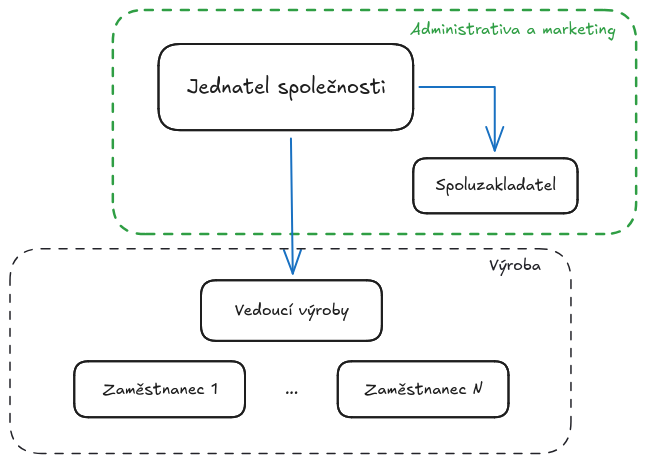
\includegraphics[width=0.8\textwidth]{files/obr1.png}
  \caption{Organizační struktura společnosti}
\end{figure}

Sídlo společnosti se nachází v Brně, konkrétně v kancelářské budově v blízkosti centra města, což usnadňuje přístup pro zaměstnance i zákazníky.
Prostor je vybavený moderními kancelářemi a výrobními dílnami pro výrobu čepic.
Orientační bod je blízkost hlavního nádraží, což usnadňuje dopravu do firmy.
K dispozici je parkování pro zaměstnance i návštěvníky, a to v areálu budovy, což zajišťuje pohodlný přístup.
\vspace{10pt}

Firma bude fungovat s malým administrativním zázemím pro správu objednávek, komunikaci s dodavateli a zákazníky.
Provozní doba firmy bude od pondělí do pátku, od 8:00 do 16:00 hodin.
V této době bude probíhat jak výroba, tak i administrativa.
Firma se zaměří na efektivní komunikaci a rychlé dodání produktů zákazníkům.

\pagebreak

\subsubsection{BOZP}

Naše firma se zaměřuje na ruční výrobu čepic pro kočky. 
Vzhledem k povaze práce je nutné zajistit bezpečné pracovní prostředí pro všechny zaměstnance. 
Hlavní rizika se týkají práce s textilními materiály, šicími stroji, ostrými nástroji a ergonomie při dlouhodobém sezení.
\vspace{10pt}

Následující rizika by měla být zohledněna v rámci BOZP(tento list není konečný, avšak obsahuje rizika s nejvyšším potenciálem poškození):

\begin{enumerate}
  \item Riziko poranění ostrými nástroji - nůžky, jehly, špendlíky.
  \item Riziko poranění šicími stroji - šití na strojích s rizikem šití prstů.
  \item Riziko úrazu elektrickým proudem - při používání elektrických strojů.
  \item Riziko vzniku požáru - při práci s hořlavými materiály.
\end{enumerate}

\vspace{10pt}

Pro předejití těmto rizikům je nutné zajistit pravidla BOZP, která budou dodržována všemi zaměstnanci.
Je nutné všechny zaměstnance seznámit s těmito pravidly a pravidelně je kontrolovat. Tento list
obsahuje základní opatření, která by měla být dodržována:

\begin{enumerate}
  \item Používání ochranných pomůcek - rukavice, brýle, roušky.
  \item Pravidelná údržba strojů a kontrola jejich bezpečnosti.
  \item Pravidelná kontrola elektrických zařízení.
  \item Důrazné proškolení zaměstnanců pro práci s elektrickými zařízeními.
  \item Umístění hasicích přístrojů a školení zaměstnanců v jejich používání.
  \item Zákaz používání otevřeného ohně(včetně kouření) v dílně.
\end{enumerate}

\subsection{Popis vyráběného výrobku}

Hats for Cats se zaměřuje na výrobu čepic pro kočky. Čepice jsou vyráběny 
z kvalitních a hypoalergenních materiálů, které jsou přizpůsobeny pohodlí a bezpečnosti zvířete.
Produkty zahrnují sezónní kolekce (zimní čepice, letní kloboučky) i tematické modely (vánoční, narozeninové, apod.),
či čepice kompletně na míru. Lze se je objednat v různých velikostech, tak aby seděly na většinu koček.

\section{Realizace}
\subsection{Výroba}

Jak již bylo zmíňeno, výroba se odehrává v prostorách firmy v Brně. 
\vspace{10pt}

Výroba čepic začíná výběrem kvalitních materiálů, které jsou jemné, elastické a bezpečné pro kočičí pokožku.
Používáme především přírodní látky jako bavlnu a vlnu, které jsou prodyšné a hypoalergenní.
Každý kus je ručně střižen, šit a dekorován našimi zkušenými zaměstnanci, kteří mají dlouholeté zkušenosti s textilní výrobou.

Výrobní proces obecně zahrnuje následující kroky:

\begin{enumerate}
  \item Výběr materiálů: Vybíráme látky, které jsou měkké a šetrné k pokožce koček.
  \item Střih a příprava: Látky jsou ručně stříhány podle předem navržených vzorců.
  \item Šití: Čepice jsou šity na šicích strojích
  \item Dekorace a dokončení: Pokud má čepice dekorace, jsou přidány ručně.
\end{enumerate}

Mezi materiály, které používáme, patří bavlna, jemná vlna a elastické tkaniny, které umožňují snadné nasazení a pohodlné nošení.

\subsubsection{Výrobní kapacita}

Výrobní kapacita firmy je závislá na počtu zaměstnanců, dostupných prostorách a poptávce.
Pro začátek se můžeme řídit následující rovnicí pro přibližný výpočet výrobní kapacity za měsíc:

\begin{equation}
  \text{Výrobní kapacita} = \text{zaměstnanci} \cdot \text{čepic za den} \cdot 20
\end{equation}

\subsection{Dodavatelé a distribuce}
\section{Charakteristika trhu}
\subsection{Zákazníci}
\subsection{Konkurence}
\section{Marketingový plán}
\section{Finanční plán}
\section{Rizika}
\section{Závěr}
\section{Seznam použité literatury}
\printbibliography[heading=none]
\section{Přílohy}

\end{document}